\documentclass[11pt, a4paper]{article}
\usepackage[utf8]{inputenc}
\usepackage{booktabs}
\usepackage{rotating}
\usepackage{hyperref}
\usepackage{color, colortbl}
\usepackage{mathtools}
\usepackage{pdfpages}
\usepackage{fourier}
\usepackage[utf8]{inputenc} % Required for inputting international characters
\usepackage[T1]{fontenc} % Output font encoding for international characters
\usepackage[parfill]{parskip}
\usepackage[left=2cm,right=2cm,top=1.5cm]{geometry}
\usepackage{tikz}
\definecolor{Gray}{gray}{0.9}
\setlength\parindent{0pt}


\begin{document}
	\pagenumbering{gobble}
\thispagestyle{empty}

\begin{center}
	\Large
	Technische Universität Dortmund\\
	Fakultät Statistik\\
	Wintersemester 2023/24\\
	
	\vspace{6em}
	
	Erhebungstechniken: Bericht über Fragebogenstudie
	
	\Huge
	\textbf{Lernortsituation an der TU Dortmund}
	
	\Large
	\vspace{4em}
	DozentInnen:	\\Prof. Dr. Philipp Doebler \\Loreen Sabel, M.Sc.\\Hannah Bartmann, B.Sc.


	\vspace{6em}
	Verfasser: \\
	Yannick Miguel \\Jacqueline Link
	
	\vspace{6em}
	Gruppenmitglieder:\\
	Johanna Hohmann\\
	Lisa Larrass
	
    \vspace{6em}
    
	31.01.2024
\end{center}

\newpage \null\thispagestyle{empty}\newpage
\tableofcontents
\newpage\null\thispagestyle{empty}\newpage
Zusammenfassung (bis zu 250 Wörter)
\newpage\null\thispagestyle{empty}\newpage

\newpage
\cleardoublepage% ensures that the page numbering will change on a recto page
\pagenumbering{arabic}
\section{Einleitung}
\label{Einleitung}
Mit dem Wegfall der Universitätsbibliothek (UB) im August 2023 stellt sich einigen Studenten die Frage: “Wo soll ich zukünftig lernen?”.
Abgesehen von den vielen Plätzen zum Lernen, ist die UB für viele von individueller Wichtigkeit.
Durch den idealen Standort und den langen Öffnungszeiten, ist die Schließung der UB für viele Studierende ein großer Verlust.
Die Technische Universität Dortmund ist bemüht Ersatz zu schaffen, eröffnet die Sebrath-Bibliothek und erweitert einige Lernorte wie den Co-Learning Space.
Unter anderem wurden auch in der Galerie und im Mensagebäude neue Lernplätze geschaffen.
Doch reichen diese Änderungen, um den Verlust der Universitätsbibliothek auszugleichen?
Gibt es genug Lernorte für die Studenten? Wie ist die Zufriedenheit mit diesen?
Ist die Situation eventuell sogar besser als vorher?

Mit all diesen wichtigen Fragen beschäftigt sich der folgende Bericht.
Anhand einer Fragebogen-Auswertung wird ein vielseitiger Einblick in die Veränderung der Lernort-Nutzung an der TU Dortmund ab dem Wintersemester 2023/24 ermöglicht.


\newpage
\section{Erhebungsinstrument}
\label{Erhebungsinstrument}
Der Fragebogen umfasst 4 Seiten und 15 Fragen und die Items wurden in 3 Partien unterteilt. wobei der erste Teil 10 Fragen zur Nutzung der Lernorte enthält, der Zweite anhand von 4 Items die Demographie befasst und der letzte Abschnitt Möglichkeit für offenes Feedback gibt.
Diese Reihenfolge sollte die Spannung aufrechterhalten und dem Ausfüllen einen roten Faden geben. 
Damit der Fragebogen übersichtlich bleibt, wurde diesen Abschnitten jeweils eine Überschrift gegeben, die unterstrichen worden ist.
Auch wurde darauf geachtet, dass das Layout einheitlich ist, indem auf jeder Seite das TU-Dortmund Logo oben zu sehen ist und Seitenzahlen unten hinzugefügt wurden.

Der Fragebogen startet mit dem Titel “Veränderung der Lernort-Nutzung an der TU Dortmund ab dem Wintersemester 2023/24” und gibt dann eine kurze Einleitung mit einer Motivation zum Thema. Zudem wird hier kurz der Rahmen der Befragung geschildert und darauf hingewiesen, für wen sich dieser Fragebogen eignet.

Der erste Teil mit der Überschrift Nutzung der Lernorte beginnt mit einer Einstiegsfrage.
Der Leser wird gefragt, ob er diese Woche bereits einen Lernort genutzt hat. Diese einfache Ja-Nein-Frage soll ihn motivieren und einen persönlichen Bezug zu dem Thema herstellen. Für die Auswertung ist dieses Item jedoch irrelevant.

Alle Items bestehen aus einer Frage und einer kursiv geschriebenen technischen Anweisung. Diese soll das Ausfüllen einfacher gestalten und den Befragten dabei unterstützen, die Fragen korrekt und zweifelsfrei beantworten zu können.

Danach wird in offener Form die Nutzungszeit der Lernorte jeweils vorher und jetzt erhoben. 

Das 3. Item besteht aus einer Tabelle und erfasst, welche Lernorte vorher und aktuell genutzt worden sind.
Um Missverständnisse zu vermeiden, wurden die Möglichkeiten für die Sebrath-Bibliothek und Universitätsbibliothek eingeschränkt, da diese vorher, bzw. jetzt nicht mehr existieren.
Mit halboffenen Antwortmöglichkeiten werden danach die Gründe für die Nutzung erfragt.

Um das Ausfüllen zu erleichtern, erstrecken sich über die zweite Seite drei inhaltlich eng gebundene Tabellen. In diesen werden hierfür vorab gewählte Aspekte auf Wichtigkeit und Umsetzung geprüft. Die zehn gewählten Aspekte sind logischerweise identisch und in allen Tabellen in der gleichen Reihenfolge.
Es wurde sich dabei für gebundene Antwortmöglichkeiten entschieden.
In der ersten Tabelle gibt es die Möglichkeit, den Aspekten eine Wichtigkeit zuzuordnen. Dies geschieht mit einer bipolaren Ratingskala der Breite fünf.
Die zwei nachfolgenden Tabellen haben das gleiche Format und ermöglichen die Bewertung der Umsetzung der Kriterien. Hier wird eine unipolaren Ratingskala genutzt, welche genau wie das Schulnotensystem aufgebaut ist, jedoch 
mit den entsprechend bekannten Begriffen verbalisiert wurde.
Dadurch sollte dem Befragten die Entscheidung einfacher fallen, da das Notensystem insbesondere für Studenten sehr intuitiv ist.
Um für Klarheit zu sorgen, welche Tabelle für Vorher und welche für Aktuell ist, wurden im Itemstamm diese Begriffe mit Fettschrift hervorgehoben.

Danach gibt es passend dazu auch die Möglichkeit, in einem halboffenen Item einen weiteren Aspekt zu nennen und diesen analog zu bewerten.
Abschließend wird im ersten Teil noch eine allgemeine Bewertung der aktuellen Lernort-Situation erfragt.
Dazu wird eine bipolare Ratingskala genutzt, die bewusst keine neutrale Antwortmöglichkeit bietet.
Um deutlich zu machen, dass es sich hier um eine Einfachnennung handelt, wurden die Ankreuzfelder hier mit Kreis gewählt.
In Frage 11 wird gefragt, ob der Ausgleich der Universitätsbibliothek angemessen ist. Diese dichotome Frage bezieht sich logischerweise nur auf Studierende, die auch die Universitätsbibliothek genutzt haben. 

Im zweiten Teil werden nun das Geschlecht und der angestrebte Studienabschluss erfragt, sowie die durchschnittliche Fahrzeit in Minuten zum Campus.
Zudem soll der Befragte in einem offenen Item seine Fakultät angeben.
Um Schwierigkeiten zu vermeiden, sollten Lehramtsstudenten die Fakultät 12 angeben.

Auf der letzten Seite gibt es dann die Möglichkeit, in einem Textfeld Feedback zu geben.
Darunter wird sich formal bedankt und es wird angegeben, wer für diesen Fragebogen verantwortlich ist.
\newpage
\section{Stichprobe und Datensatz}
\label{Stichprobe und Datensatz}

Die Daten wurden auf dem Campus der Technischen Universität Dortmund, vor allem an diversen Lernorten, erhoben. Die Orte der Erhebung wurde zudem auch als Meta-Daten notiert. Dabei fällt auf, dass vermehrt im Mathetower und der Galerie befragt wurde (jeweils ca. 30).

Die Personen wurden zunächst gefragt, ob sie mindestens seit dem Sommersemester 2023 an der TU Dortmund studieren. Falls dies der Fall war, wurde ihnen der Fragebogen ausgehändigt. Dieser wurde dann schriftlich ohne Einwirkungen des Interviewers ausgefüllt. Gegebenenfalls wurde auf Rückfragen eingegangen.
Die Erhebung erfolgte nicht nur an unterschiedlichen Orten, sondern auch an unterschiedlichen Tageszeiten, sowie Wochentagen, um ein diverses Meinungsbild zu erlangen.

Die Grundgesamtheit setzt sich aus allen Studierenden der Technischen Universität Dortmund zusammen, die mindestens seit dem Sommersemester 2023 studieren. Das heißt, es handelt sich um eine Grundgesamtheit von 25 169 Personen. 
Es wurden 141 Fragebögen erhoben, wobei davon 138 verwertbar waren. Zwei Fragebögen wurden entfernt, da diese leer abgegeben wurden. Des Weiteren hat eine Person erst seit dem Wintersemester 2024 studiert. Dieser Fragebogen wurde ebenfalls aussortiert.
Die Stichprobe besteht daher aus 138 Studierenden.

Bezüglich der Verteilung der Geschlechter fällt auf, dass weiblich sowie männlich identifizierende Personen ungefähr gleich häufig erhoben wurden. Zusätzlich gab es noch zwei divers-identifizierende Personen. 
117 Studierende gaben an, dass sie sich im Bachelor befinden. Hingegen gaben 19 an, dass sie sich im Master befinden. Es ist zu erkennen, dass mehr Studierende im Bachelor befragt wurden. zahlen vergleich online
Außerdem wurden die Fakultäten erfasst. Dabei wurde jede Fakultät außer Fakultät 17 erfasst. Insgesamt gaben 30 Befragte an, an der Fakultät 5 (Statistik) zu studieren und ebenfalls 30, dass sie an der Fakultät 12 (Erziehungswissenschaften, Psychologie und Bildungsforschung) studieren. Die restlichen Befragten sind unter den anderen 14 Fakultäten etwa gleichmäßig verteilt. (siehe dazu auch Anhang)

Die Dateneingabe erfolgte über ein gemeinsames Excel-Dokument. Jedes Gruppenmitglied hat dabei eine eigene Tabelle genutzt, die einem vorgegebenen Prototyp entsprach. Eine einheitliche Kodierung erfolgte mithilfe einer Kodierungshilfe. 
Zur Datenauswertung und -analyse wurden die vier Tabellen dann zu einer einzelnen Excel-Tabelle zusammengefügt. 
Bei Frage 3 zur Nutzung von Lernorten wurde eine angekreuzte Antwort, also ein Ja, als Eins kodiert bzw. ein leeres Feld, daher Nein, als eine Null. Ebenso geschah dies bei Frage 4, wofür die Lernorte genutzt werden, bzw. Frage 9, bezüglich der Ersatzbewertung.
Bei den Fragen 6 bis 7, welche sich mit der Bewertung der Aspekte der Lernumgebung beschäftigen, wurden die verbalisierten Schulnoten umkodiert zu Zahlen von 1 bis 6. Ebenso wurde “Sehr unwichtig” bis “sehr wichtig” umkodiert zu 1 bis 5.
Die ordinalskalierten Daten, also aus den Fragen 5 bis 9, wurden bei der weiteren Auswertung orientiert an dieser Kodierung quasi-intervallskaliert behandelt.
Bei den personenbezogenen Daten wurde bei dem Geschlecht “weiblich” zu 1 umkodiert, “männlich” zu 2 und “divers” zu 3. 
Bei der Angabe zum Studium wurde “Bachelor” zu 1, “Master” zu 2 und “Nein” zu 0. Die Fragebögen, bei denen daher eine 0 erfasst wurde, wurden aussortiert.
Sollte es bei der Fahrtzeit dazu gekommen sein, dass die Angabge als  angegeben wurde, wurde das arithmetische Mittel berechnet.

Für die latente Variable "Gesamtzufriedenheit" haben wir folgende Formel aufgestellt:  \\
Der "Score" berechnet sich aus:
\begin{equation*}
	z_i = \frac{\sum\limits_{j=1}^{10}x_{ij}\cdot  y_{ij}}{\sum\limits_{j=1}^{10}x_{ij}} \hspace{0.8cm} , \text{für} \ 
	i=1,...,138\  \text{und} \ j=1,...,10
\end{equation*} 
Dabei ist $z_i$ der Score der i-ten Person. \\
$x_{ij}$ ist die Wichtigkeit des j-ten Aspekts der i-ten Person und
$y_{ij}$ ist die Bewertung der Umsetzung des j-ten Aspekts der i-ten Person.


Dies geschieht jeweils für den Zeitraum vor dem Wintersemester 2024 und einmal für die Beurteilung ab Beginn des Wintersemesters 2024. Daher ergibt sich dann ein Score-Vorher sowie ein Score-Nachher. Bei den Scores handelt es sich um latente Variablen.

Zuzüglich der beiden Scores wurden insgesamt 70 Variablen erfasst.
Die ordinalskalierten Daten, also aus den Fragen 5 bis 9, wurden bei der weiteren Auswertung quasi-intervallskaliert behandelt.

\newpage
\begin{figure}
\centering % Created by tikzDevice version 0.12.5 on 2024-01-20 15:22:02
% !TEX encoding = UTF-8 Unicode
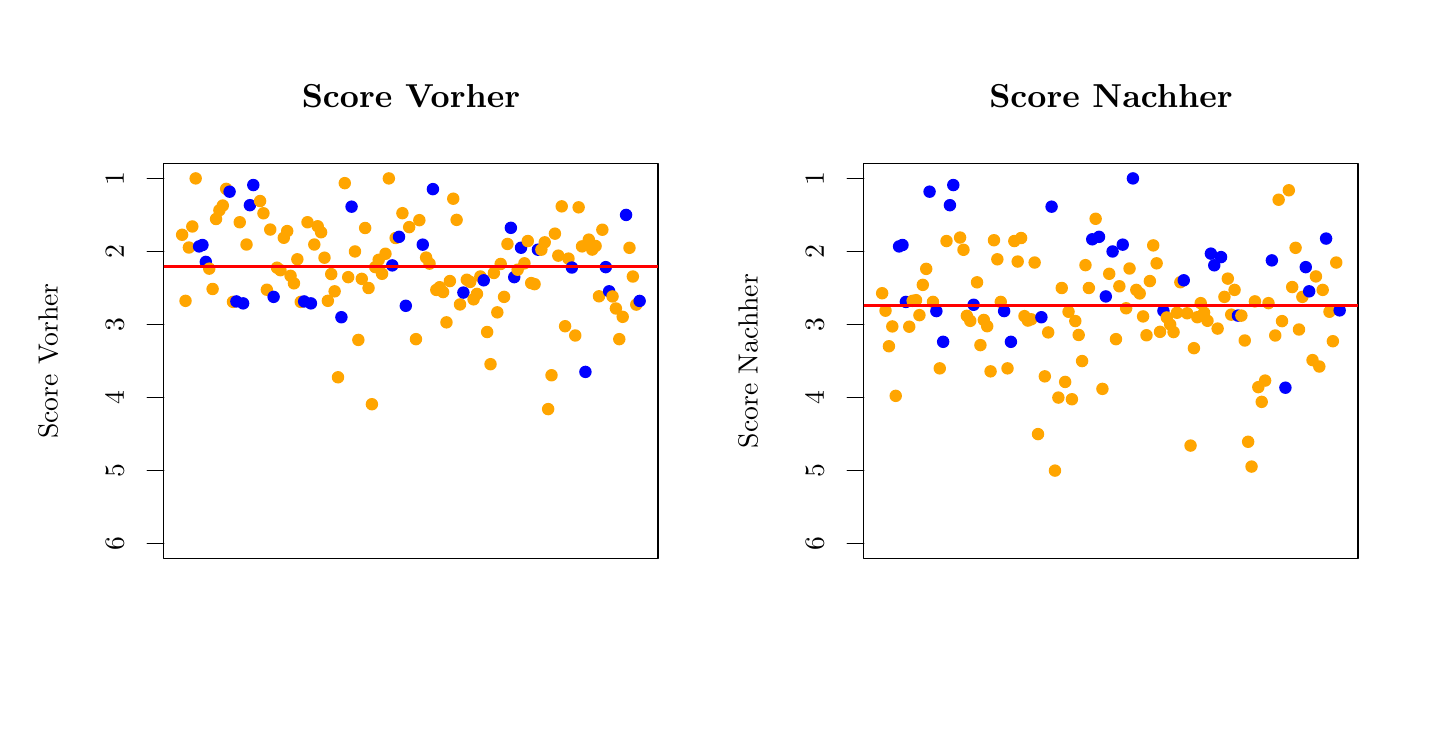
\begin{tikzpicture}[x=1pt,y=1pt]
\definecolor{fillColor}{RGB}{255,255,255}
\path[use as bounding box,fill=fillColor,fill opacity=0.00] (0,0) rectangle (505.89,252.94);
\begin{scope}
\path[clip] ( 49.20, 61.20) rectangle (227.75,203.75);
\definecolor{fillColor}{RGB}{255,165,0}

\path[fill=fillColor] ( 55.81,178.10) circle (  2.25);

\path[fill=fillColor] ( 57.04,154.23) circle (  2.25);

\path[fill=fillColor] ( 58.26,173.50) circle (  2.25);

\path[fill=fillColor] ( 59.49,181.10) circle (  2.25);

\path[fill=fillColor] ( 60.71,198.47) circle (  2.25);
\definecolor{fillColor}{RGB}{0,0,255}

\path[fill=fillColor] ( 61.94,173.89) circle (  2.25);

\path[fill=fillColor] ( 63.16,174.40) circle (  2.25);

\path[fill=fillColor] ( 64.38,168.30) circle (  2.25);
\definecolor{fillColor}{RGB}{255,165,0}

\path[fill=fillColor] ( 65.61,165.86) circle (  2.25);

\path[fill=fillColor] ( 66.83,158.51) circle (  2.25);

\path[fill=fillColor] ( 68.06,183.80) circle (  2.25);

\path[fill=fillColor] ( 69.28,186.96) circle (  2.25);

\path[fill=fillColor] ( 70.51,188.66) circle (  2.25);

\path[fill=fillColor] ( 71.73,194.69) circle (  2.25);
\definecolor{fillColor}{RGB}{0,0,255}

\path[fill=fillColor] ( 72.96,193.67) circle (  2.25);
\definecolor{fillColor}{RGB}{255,165,0}

\path[fill=fillColor] ( 74.18,153.84) circle (  2.25);
\definecolor{fillColor}{RGB}{0,0,255}

\path[fill=fillColor] ( 75.41,154.01) circle (  2.25);
\definecolor{fillColor}{RGB}{255,165,0}

\path[fill=fillColor] ( 76.63,182.63) circle (  2.25);
\definecolor{fillColor}{RGB}{0,0,255}

\path[fill=fillColor] ( 77.86,153.31) circle (  2.25);
\definecolor{fillColor}{RGB}{255,165,0}

\path[fill=fillColor] ( 79.08,174.58) circle (  2.25);
\definecolor{fillColor}{RGB}{0,0,255}

\path[fill=fillColor] ( 80.30,188.79) circle (  2.25);

\path[fill=fillColor] ( 81.53,196.07) circle (  2.25);
\definecolor{fillColor}{RGB}{255,165,0}

\path[fill=fillColor] ( 83.98,190.29) circle (  2.25);

\path[fill=fillColor] ( 85.20,185.87) circle (  2.25);

\path[fill=fillColor] ( 86.43,158.24) circle (  2.25);

\path[fill=fillColor] ( 87.65,179.99) circle (  2.25);
\definecolor{fillColor}{RGB}{0,0,255}

\path[fill=fillColor] ( 88.88,155.66) circle (  2.25);
\definecolor{fillColor}{RGB}{255,165,0}

\path[fill=fillColor] ( 90.10,166.20) circle (  2.25);

\path[fill=fillColor] ( 91.33,165.30) circle (  2.25);

\path[fill=fillColor] ( 92.55,177.02) circle (  2.25);

\path[fill=fillColor] ( 93.78,179.44) circle (  2.25);

\path[fill=fillColor] ( 95.00,163.27) circle (  2.25);

\path[fill=fillColor] ( 96.22,160.56) circle (  2.25);

\path[fill=fillColor] ( 97.45,169.24) circle (  2.25);

\path[fill=fillColor] ( 98.67,153.84) circle (  2.25);
\definecolor{fillColor}{RGB}{0,0,255}

\path[fill=fillColor] ( 99.90,154.01) circle (  2.25);
\definecolor{fillColor}{RGB}{255,165,0}

\path[fill=fillColor] (101.12,182.63) circle (  2.25);
\definecolor{fillColor}{RGB}{0,0,255}

\path[fill=fillColor] (102.35,153.31) circle (  2.25);
\definecolor{fillColor}{RGB}{255,165,0}

\path[fill=fillColor] (103.57,174.58) circle (  2.25);

\path[fill=fillColor] (104.80,181.17) circle (  2.25);

\path[fill=fillColor] (106.02,179.01) circle (  2.25);

\path[fill=fillColor] (107.25,169.81) circle (  2.25);

\path[fill=fillColor] (108.47,154.23) circle (  2.25);

\path[fill=fillColor] (109.69,163.90) circle (  2.25);

\path[fill=fillColor] (110.92,157.67) circle (  2.25);

\path[fill=fillColor] (112.14,126.61) circle (  2.25);
\definecolor{fillColor}{RGB}{0,0,255}

\path[fill=fillColor] (113.37,148.31) circle (  2.25);
\definecolor{fillColor}{RGB}{255,165,0}

\path[fill=fillColor] (114.59,196.76) circle (  2.25);

\path[fill=fillColor] (115.82,162.79) circle (  2.25);
\definecolor{fillColor}{RGB}{0,0,255}

\path[fill=fillColor] (117.04,188.25) circle (  2.25);
\definecolor{fillColor}{RGB}{255,165,0}

\path[fill=fillColor] (118.27,172.07) circle (  2.25);

\path[fill=fillColor] (119.49,140.11) circle (  2.25);

\path[fill=fillColor] (120.72,162.17) circle (  2.25);

\path[fill=fillColor] (121.94,180.55) circle (  2.25);

\path[fill=fillColor] (123.17,158.87) circle (  2.25);

\path[fill=fillColor] (124.39,116.87) circle (  2.25);

\path[fill=fillColor] (125.61,166.41) circle (  2.25);

\path[fill=fillColor] (126.84,169.05) circle (  2.25);

\path[fill=fillColor] (128.06,164.00) circle (  2.25);

\path[fill=fillColor] (129.29,171.24) circle (  2.25);

\path[fill=fillColor] (130.51,198.47) circle (  2.25);
\definecolor{fillColor}{RGB}{0,0,255}

\path[fill=fillColor] (131.74,167.04) circle (  2.25);
\definecolor{fillColor}{RGB}{255,165,0}

\path[fill=fillColor] (132.96,176.93) circle (  2.25);
\definecolor{fillColor}{RGB}{0,0,255}

\path[fill=fillColor] (134.19,177.35) circle (  2.25);
\definecolor{fillColor}{RGB}{255,165,0}

\path[fill=fillColor] (135.41,185.90) circle (  2.25);
\definecolor{fillColor}{RGB}{0,0,255}

\path[fill=fillColor] (136.64,152.44) circle (  2.25);
\definecolor{fillColor}{RGB}{255,165,0}

\path[fill=fillColor] (137.86,180.87) circle (  2.25);

\path[fill=fillColor] (140.31,140.39) circle (  2.25);

\path[fill=fillColor] (141.53,183.38) circle (  2.25);
\definecolor{fillColor}{RGB}{0,0,255}

\path[fill=fillColor] (142.76,174.54) circle (  2.25);
\definecolor{fillColor}{RGB}{255,165,0}

\path[fill=fillColor] (143.98,169.87) circle (  2.25);

\path[fill=fillColor] (145.21,167.67) circle (  2.25);
\definecolor{fillColor}{RGB}{0,0,255}

\path[fill=fillColor] (146.43,194.60) circle (  2.25);
\definecolor{fillColor}{RGB}{255,165,0}

\path[fill=fillColor] (147.66,158.18) circle (  2.25);

\path[fill=fillColor] (148.88,159.15) circle (  2.25);

\path[fill=fillColor] (150.11,157.40) circle (  2.25);

\path[fill=fillColor] (151.33,146.45) circle (  2.25);

\path[fill=fillColor] (152.56,161.37) circle (  2.25);

\path[fill=fillColor] (153.78,191.13) circle (  2.25);

\path[fill=fillColor] (155.00,183.48) circle (  2.25);

\path[fill=fillColor] (156.23,152.93) circle (  2.25);
\definecolor{fillColor}{RGB}{0,0,255}

\path[fill=fillColor] (157.45,157.22) circle (  2.25);
\definecolor{fillColor}{RGB}{255,165,0}

\path[fill=fillColor] (158.68,161.85) circle (  2.25);

\path[fill=fillColor] (159.90,161.07) circle (  2.25);

\path[fill=fillColor] (161.13,154.77) circle (  2.25);

\path[fill=fillColor] (162.35,156.74) circle (  2.25);

\path[fill=fillColor] (163.58,163.04) circle (  2.25);
\definecolor{fillColor}{RGB}{0,0,255}

\path[fill=fillColor] (164.80,161.65) circle (  2.25);
\definecolor{fillColor}{RGB}{255,165,0}

\path[fill=fillColor] (166.03,142.96) circle (  2.25);

\path[fill=fillColor] (167.25,131.34) circle (  2.25);

\path[fill=fillColor] (168.47,164.30) circle (  2.25);

\path[fill=fillColor] (169.70,150.07) circle (  2.25);

\path[fill=fillColor] (170.92,167.56) circle (  2.25);

\path[fill=fillColor] (172.15,155.66) circle (  2.25);

\path[fill=fillColor] (173.37,174.78) circle (  2.25);
\definecolor{fillColor}{RGB}{0,0,255}

\path[fill=fillColor] (174.60,180.61) circle (  2.25);

\path[fill=fillColor] (175.82,162.79) circle (  2.25);
\definecolor{fillColor}{RGB}{255,165,0}

\path[fill=fillColor] (177.05,165.47) circle (  2.25);
\definecolor{fillColor}{RGB}{0,0,255}

\path[fill=fillColor] (178.27,173.42) circle (  2.25);
\definecolor{fillColor}{RGB}{255,165,0}

\path[fill=fillColor] (179.50,167.79) circle (  2.25);

\path[fill=fillColor] (180.72,175.84) circle (  2.25);

\path[fill=fillColor] (181.95,160.65) circle (  2.25);

\path[fill=fillColor] (183.17,160.26) circle (  2.25);
\definecolor{fillColor}{RGB}{0,0,255}

\path[fill=fillColor] (184.39,172.71) circle (  2.25);
\definecolor{fillColor}{RGB}{255,165,0}

\path[fill=fillColor] (185.62,172.71) circle (  2.25);

\path[fill=fillColor] (186.84,175.37) circle (  2.25);

\path[fill=fillColor] (188.07,115.11) circle (  2.25);

\path[fill=fillColor] (189.29,127.34) circle (  2.25);

\path[fill=fillColor] (190.52,178.51) circle (  2.25);

\path[fill=fillColor] (191.74,170.56) circle (  2.25);

\path[fill=fillColor] (192.97,188.37) circle (  2.25);

\path[fill=fillColor] (194.19,145.06) circle (  2.25);

\path[fill=fillColor] (195.42,169.49) circle (  2.25);
\definecolor{fillColor}{RGB}{0,0,255}

\path[fill=fillColor] (196.64,166.27) circle (  2.25);
\definecolor{fillColor}{RGB}{255,165,0}

\path[fill=fillColor] (197.87,141.71) circle (  2.25);

\path[fill=fillColor] (199.09,188.02) circle (  2.25);

\path[fill=fillColor] (200.31,173.91) circle (  2.25);
\definecolor{fillColor}{RGB}{0,0,255}

\path[fill=fillColor] (201.54,128.55) circle (  2.25);
\definecolor{fillColor}{RGB}{255,165,0}

\path[fill=fillColor] (202.76,176.35) circle (  2.25);

\path[fill=fillColor] (203.99,172.75) circle (  2.25);

\path[fill=fillColor] (205.21,174.05) circle (  2.25);

\path[fill=fillColor] (206.44,155.87) circle (  2.25);

\path[fill=fillColor] (207.66,179.92) circle (  2.25);
\definecolor{fillColor}{RGB}{0,0,255}

\path[fill=fillColor] (208.89,166.41) circle (  2.25);

\path[fill=fillColor] (210.11,157.67) circle (  2.25);
\definecolor{fillColor}{RGB}{255,165,0}

\path[fill=fillColor] (211.34,155.82) circle (  2.25);

\path[fill=fillColor] (212.56,151.47) circle (  2.25);

\path[fill=fillColor] (213.78,140.39) circle (  2.25);

\path[fill=fillColor] (215.01,148.45) circle (  2.25);
\definecolor{fillColor}{RGB}{0,0,255}

\path[fill=fillColor] (216.23,185.27) circle (  2.25);
\definecolor{fillColor}{RGB}{255,165,0}

\path[fill=fillColor] (217.46,173.39) circle (  2.25);

\path[fill=fillColor] (218.68,163.02) circle (  2.25);

\path[fill=fillColor] (219.91,152.87) circle (  2.25);
\definecolor{fillColor}{RGB}{0,0,255}

\path[fill=fillColor] (221.13,154.19) circle (  2.25);
\end{scope}
\begin{scope}
\path[clip] (  0.00,  0.00) rectangle (505.89,252.94);
\definecolor{drawColor}{RGB}{0,0,0}

\path[draw=drawColor,line width= 0.4pt,line join=round,line cap=round] ( 49.20,198.47) -- ( 49.20, 66.48);

\path[draw=drawColor,line width= 0.4pt,line join=round,line cap=round] ( 49.20,198.47) -- ( 43.20,198.47);

\path[draw=drawColor,line width= 0.4pt,line join=round,line cap=round] ( 49.20,172.07) -- ( 43.20,172.07);

\path[draw=drawColor,line width= 0.4pt,line join=round,line cap=round] ( 49.20,145.67) -- ( 43.20,145.67);

\path[draw=drawColor,line width= 0.4pt,line join=round,line cap=round] ( 49.20,119.27) -- ( 43.20,119.27);

\path[draw=drawColor,line width= 0.4pt,line join=round,line cap=round] ( 49.20, 92.88) -- ( 43.20, 92.88);

\path[draw=drawColor,line width= 0.4pt,line join=round,line cap=round] ( 49.20, 66.48) -- ( 43.20, 66.48);

\node[text=drawColor,rotate= 90.00,anchor=base,inner sep=0pt, outer sep=0pt, scale=  1.00] at ( 34.80, 66.48) {6};

\node[text=drawColor,rotate= 90.00,anchor=base,inner sep=0pt, outer sep=0pt, scale=  1.00] at ( 34.80, 92.88) {5};

\node[text=drawColor,rotate= 90.00,anchor=base,inner sep=0pt, outer sep=0pt, scale=  1.00] at ( 34.80,119.27) {4};

\node[text=drawColor,rotate= 90.00,anchor=base,inner sep=0pt, outer sep=0pt, scale=  1.00] at ( 34.80,145.67) {3};

\node[text=drawColor,rotate= 90.00,anchor=base,inner sep=0pt, outer sep=0pt, scale=  1.00] at ( 34.80,172.07) {2};

\node[text=drawColor,rotate= 90.00,anchor=base,inner sep=0pt, outer sep=0pt, scale=  1.00] at ( 34.80,198.47) {1};

\path[draw=drawColor,line width= 0.4pt,line join=round,line cap=round] ( 49.20, 61.20) --
	(227.75, 61.20) --
	(227.75,203.75) --
	( 49.20,203.75) --
	cycle;
\end{scope}
\begin{scope}
\path[clip] (  0.00,  0.00) rectangle (252.94,252.94);
\definecolor{drawColor}{RGB}{0,0,0}

\node[text=drawColor,anchor=base,inner sep=0pt, outer sep=0pt, scale=  1.20] at (138.47,224.20) {\bfseries Score Vorher};

\node[text=drawColor,rotate= 90.00,anchor=base,inner sep=0pt, outer sep=0pt, scale=  1.00] at ( 10.80,132.47) {Score Vorher};
\end{scope}
\begin{scope}
\path[clip] ( 49.20, 61.20) rectangle (227.75,203.75);
\definecolor{drawColor}{RGB}{255,0,0}

\path[draw=drawColor,line width= 1.2pt,line join=round,line cap=round] ( 49.20,166.62) -- (227.74,166.62);
\end{scope}
\begin{scope}
\path[clip] (302.14, 61.20) rectangle (480.69,203.75);
\definecolor{fillColor}{RGB}{255,165,0}

\path[fill=fillColor] (308.76,156.98) circle (  2.25);

\path[fill=fillColor] (309.98,150.67) circle (  2.25);

\path[fill=fillColor] (311.21,137.82) circle (  2.25);

\path[fill=fillColor] (312.43,144.98) circle (  2.25);

\path[fill=fillColor] (313.66,119.90) circle (  2.25);
\definecolor{fillColor}{RGB}{0,0,255}

\path[fill=fillColor] (314.88,173.89) circle (  2.25);

\path[fill=fillColor] (316.11,174.40) circle (  2.25);

\path[fill=fillColor] (317.33,153.84) circle (  2.25);
\definecolor{fillColor}{RGB}{255,165,0}

\path[fill=fillColor] (318.55,144.89) circle (  2.25);

\path[fill=fillColor] (319.78,154.23) circle (  2.25);

\path[fill=fillColor] (321.00,154.47) circle (  2.25);

\path[fill=fillColor] (322.23,149.06) circle (  2.25);

\path[fill=fillColor] (323.45,160.00) circle (  2.25);

\path[fill=fillColor] (324.68,165.78) circle (  2.25);
\definecolor{fillColor}{RGB}{0,0,255}

\path[fill=fillColor] (325.90,193.67) circle (  2.25);
\definecolor{fillColor}{RGB}{255,165,0}

\path[fill=fillColor] (327.13,153.84) circle (  2.25);
\definecolor{fillColor}{RGB}{0,0,255}

\path[fill=fillColor] (328.35,150.53) circle (  2.25);
\definecolor{fillColor}{RGB}{255,165,0}

\path[fill=fillColor] (329.58,129.83) circle (  2.25);
\definecolor{fillColor}{RGB}{0,0,255}

\path[fill=fillColor] (330.80,139.42) circle (  2.25);
\definecolor{fillColor}{RGB}{255,165,0}

\path[fill=fillColor] (332.02,175.84) circle (  2.25);
\definecolor{fillColor}{RGB}{0,0,255}

\path[fill=fillColor] (333.25,188.79) circle (  2.25);

\path[fill=fillColor] (334.47,196.07) circle (  2.25);
\definecolor{fillColor}{RGB}{255,165,0}

\path[fill=fillColor] (336.92,177.10) circle (  2.25);

\path[fill=fillColor] (338.15,172.67) circle (  2.25);

\path[fill=fillColor] (339.37,148.81) circle (  2.25);

\path[fill=fillColor] (340.60,146.99) circle (  2.25);
\definecolor{fillColor}{RGB}{0,0,255}

\path[fill=fillColor] (341.82,152.81) circle (  2.25);
\definecolor{fillColor}{RGB}{255,165,0}

\path[fill=fillColor] (343.05,160.92) circle (  2.25);

\path[fill=fillColor] (344.27,138.23) circle (  2.25);

\path[fill=fillColor] (345.50,147.32) circle (  2.25);

\path[fill=fillColor] (346.72,145.06) circle (  2.25);

\path[fill=fillColor] (347.94,128.75) circle (  2.25);

\path[fill=fillColor] (349.17,176.13) circle (  2.25);

\path[fill=fillColor] (350.39,169.24) circle (  2.25);

\path[fill=fillColor] (351.62,153.84) circle (  2.25);
\definecolor{fillColor}{RGB}{0,0,255}

\path[fill=fillColor] (352.84,150.53) circle (  2.25);
\definecolor{fillColor}{RGB}{255,165,0}

\path[fill=fillColor] (354.07,129.83) circle (  2.25);
\definecolor{fillColor}{RGB}{0,0,255}

\path[fill=fillColor] (355.29,139.42) circle (  2.25);
\definecolor{fillColor}{RGB}{255,165,0}

\path[fill=fillColor] (356.52,175.84) circle (  2.25);

\path[fill=fillColor] (357.74,168.43) circle (  2.25);

\path[fill=fillColor] (358.97,176.93) circle (  2.25);

\path[fill=fillColor] (360.19,148.69) circle (  2.25);

\path[fill=fillColor] (361.42,147.10) circle (  2.25);

\path[fill=fillColor] (362.64,147.56) circle (  2.25);

\path[fill=fillColor] (363.86,168.07) circle (  2.25);

\path[fill=fillColor] (365.09,106.08) circle (  2.25);
\definecolor{fillColor}{RGB}{0,0,255}

\path[fill=fillColor] (366.31,148.31) circle (  2.25);
\definecolor{fillColor}{RGB}{255,165,0}

\path[fill=fillColor] (367.54,126.94) circle (  2.25);

\path[fill=fillColor] (368.76,142.82) circle (  2.25);
\definecolor{fillColor}{RGB}{0,0,255}

\path[fill=fillColor] (369.99,188.25) circle (  2.25);
\definecolor{fillColor}{RGB}{255,165,0}

\path[fill=fillColor] (371.21, 92.88) circle (  2.25);

\path[fill=fillColor] (372.44,119.27) circle (  2.25);

\path[fill=fillColor] (373.66,158.87) circle (  2.25);

\path[fill=fillColor] (374.89,124.93) circle (  2.25);

\path[fill=fillColor] (376.11,150.29) circle (  2.25);

\path[fill=fillColor] (377.33,118.67) circle (  2.25);

\path[fill=fillColor] (378.56,146.93) circle (  2.25);

\path[fill=fillColor] (379.78,141.90) circle (  2.25);

\path[fill=fillColor] (381.01,132.47) circle (  2.25);

\path[fill=fillColor] (382.23,167.12) circle (  2.25);

\path[fill=fillColor] (383.46,158.87) circle (  2.25);
\definecolor{fillColor}{RGB}{0,0,255}

\path[fill=fillColor] (384.68,176.47) circle (  2.25);
\definecolor{fillColor}{RGB}{255,165,0}

\path[fill=fillColor] (385.91,183.88) circle (  2.25);
\definecolor{fillColor}{RGB}{0,0,255}

\path[fill=fillColor] (387.13,177.35) circle (  2.25);
\definecolor{fillColor}{RGB}{255,165,0}

\path[fill=fillColor] (388.36,122.42) circle (  2.25);
\definecolor{fillColor}{RGB}{0,0,255}

\path[fill=fillColor] (389.58,155.82) circle (  2.25);
\definecolor{fillColor}{RGB}{255,165,0}

\path[fill=fillColor] (390.81,164.00) circle (  2.25);
\definecolor{fillColor}{RGB}{0,0,255}

\path[fill=fillColor] (392.03,172.07) circle (  2.25);
\definecolor{fillColor}{RGB}{255,165,0}

\path[fill=fillColor] (393.25,140.39) circle (  2.25);

\path[fill=fillColor] (394.48,159.50) circle (  2.25);
\definecolor{fillColor}{RGB}{0,0,255}

\path[fill=fillColor] (395.70,174.54) circle (  2.25);
\definecolor{fillColor}{RGB}{255,165,0}

\path[fill=fillColor] (396.93,151.54) circle (  2.25);

\path[fill=fillColor] (398.15,165.91) circle (  2.25);
\definecolor{fillColor}{RGB}{0,0,255}

\path[fill=fillColor] (399.38,198.47) circle (  2.25);
\definecolor{fillColor}{RGB}{255,165,0}

\path[fill=fillColor] (400.60,158.18) circle (  2.25);

\path[fill=fillColor] (401.83,156.90) circle (  2.25);

\path[fill=fillColor] (403.05,148.60) circle (  2.25);

\path[fill=fillColor] (404.28,141.79) circle (  2.25);

\path[fill=fillColor] (405.50,161.37) circle (  2.25);

\path[fill=fillColor] (406.72,174.27) circle (  2.25);

\path[fill=fillColor] (407.95,167.79) circle (  2.25);

\path[fill=fillColor] (409.17,143.03) circle (  2.25);
\definecolor{fillColor}{RGB}{0,0,255}

\path[fill=fillColor] (410.40,150.62) circle (  2.25);
\definecolor{fillColor}{RGB}{255,165,0}

\path[fill=fillColor] (411.62,148.23) circle (  2.25);

\path[fill=fillColor] (412.85,145.67) circle (  2.25);

\path[fill=fillColor] (414.07,142.94) circle (  2.25);

\path[fill=fillColor] (415.30,149.93) circle (  2.25);

\path[fill=fillColor] (416.52,160.95) circle (  2.25);
\definecolor{fillColor}{RGB}{0,0,255}

\path[fill=fillColor] (417.75,161.65) circle (  2.25);
\definecolor{fillColor}{RGB}{255,165,0}

\path[fill=fillColor] (418.97,149.73) circle (  2.25);

\path[fill=fillColor] (420.20,101.93) circle (  2.25);

\path[fill=fillColor] (421.42,137.13) circle (  2.25);

\path[fill=fillColor] (422.64,148.31) circle (  2.25);

\path[fill=fillColor] (423.87,153.40) circle (  2.25);

\path[fill=fillColor] (425.09,149.95) circle (  2.25);

\path[fill=fillColor] (426.32,147.02) circle (  2.25);
\definecolor{fillColor}{RGB}{0,0,255}

\path[fill=fillColor] (427.54,171.29) circle (  2.25);

\path[fill=fillColor] (428.77,167.07) circle (  2.25);
\definecolor{fillColor}{RGB}{255,165,0}

\path[fill=fillColor] (429.99,144.20) circle (  2.25);
\definecolor{fillColor}{RGB}{0,0,255}

\path[fill=fillColor] (431.22,170.04) circle (  2.25);
\definecolor{fillColor}{RGB}{255,165,0}

\path[fill=fillColor] (432.44,155.66) circle (  2.25);

\path[fill=fillColor] (433.67,162.26) circle (  2.25);

\path[fill=fillColor] (434.89,149.24) circle (  2.25);

\path[fill=fillColor] (436.11,158.18) circle (  2.25);
\definecolor{fillColor}{RGB}{0,0,255}

\path[fill=fillColor] (437.34,148.89) circle (  2.25);
\definecolor{fillColor}{RGB}{255,165,0}

\path[fill=fillColor] (438.56,148.89) circle (  2.25);

\path[fill=fillColor] (439.79,139.90) circle (  2.25);

\path[fill=fillColor] (441.01,103.30) circle (  2.25);

\path[fill=fillColor] (442.24, 94.34) circle (  2.25);

\path[fill=fillColor] (443.46,154.04) circle (  2.25);

\path[fill=fillColor] (444.69,123.04) circle (  2.25);

\path[fill=fillColor] (445.91,117.72) circle (  2.25);

\path[fill=fillColor] (447.14,125.41) circle (  2.25);

\path[fill=fillColor] (448.36,153.40) circle (  2.25);
\definecolor{fillColor}{RGB}{0,0,255}

\path[fill=fillColor] (449.59,168.85) circle (  2.25);
\definecolor{fillColor}{RGB}{255,165,0}

\path[fill=fillColor] (450.81,141.71) circle (  2.25);

\path[fill=fillColor] (452.03,190.77) circle (  2.25);

\path[fill=fillColor] (453.26,146.90) circle (  2.25);
\definecolor{fillColor}{RGB}{0,0,255}

\path[fill=fillColor] (454.48,122.84) circle (  2.25);
\definecolor{fillColor}{RGB}{255,165,0}

\path[fill=fillColor] (455.71,194.18) circle (  2.25);

\path[fill=fillColor] (456.93,159.21) circle (  2.25);

\path[fill=fillColor] (458.16,173.39) circle (  2.25);

\path[fill=fillColor] (459.38,143.87) circle (  2.25);

\path[fill=fillColor] (460.61,155.66) circle (  2.25);
\definecolor{fillColor}{RGB}{0,0,255}

\path[fill=fillColor] (461.83,166.41) circle (  2.25);

\path[fill=fillColor] (463.06,157.67) circle (  2.25);
\definecolor{fillColor}{RGB}{255,165,0}

\path[fill=fillColor] (464.28,132.81) circle (  2.25);

\path[fill=fillColor] (465.51,163.05) circle (  2.25);

\path[fill=fillColor] (466.73,130.49) circle (  2.25);

\path[fill=fillColor] (467.95,158.18) circle (  2.25);
\definecolor{fillColor}{RGB}{0,0,255}

\path[fill=fillColor] (469.18,176.73) circle (  2.25);
\definecolor{fillColor}{RGB}{255,165,0}

\path[fill=fillColor] (470.40,150.29) circle (  2.25);

\path[fill=fillColor] (471.63,139.64) circle (  2.25);

\path[fill=fillColor] (472.85,168.07) circle (  2.25);
\definecolor{fillColor}{RGB}{0,0,255}

\path[fill=fillColor] (474.08,150.78) circle (  2.25);
\end{scope}
\begin{scope}
\path[clip] (  0.00,  0.00) rectangle (505.89,252.94);
\definecolor{drawColor}{RGB}{0,0,0}

\path[draw=drawColor,line width= 0.4pt,line join=round,line cap=round] (302.14,198.47) -- (302.14, 66.48);

\path[draw=drawColor,line width= 0.4pt,line join=round,line cap=round] (302.14,198.47) -- (296.14,198.47);

\path[draw=drawColor,line width= 0.4pt,line join=round,line cap=round] (302.14,172.07) -- (296.14,172.07);

\path[draw=drawColor,line width= 0.4pt,line join=round,line cap=round] (302.14,145.67) -- (296.14,145.67);

\path[draw=drawColor,line width= 0.4pt,line join=round,line cap=round] (302.14,119.27) -- (296.14,119.27);

\path[draw=drawColor,line width= 0.4pt,line join=round,line cap=round] (302.14, 92.88) -- (296.14, 92.88);

\path[draw=drawColor,line width= 0.4pt,line join=round,line cap=round] (302.14, 66.48) -- (296.14, 66.48);

\node[text=drawColor,rotate= 90.00,anchor=base,inner sep=0pt, outer sep=0pt, scale=  1.00] at (287.75, 66.48) {6};

\node[text=drawColor,rotate= 90.00,anchor=base,inner sep=0pt, outer sep=0pt, scale=  1.00] at (287.75, 92.88) {5};

\node[text=drawColor,rotate= 90.00,anchor=base,inner sep=0pt, outer sep=0pt, scale=  1.00] at (287.75,119.27) {4};

\node[text=drawColor,rotate= 90.00,anchor=base,inner sep=0pt, outer sep=0pt, scale=  1.00] at (287.75,145.67) {3};

\node[text=drawColor,rotate= 90.00,anchor=base,inner sep=0pt, outer sep=0pt, scale=  1.00] at (287.75,172.07) {2};

\node[text=drawColor,rotate= 90.00,anchor=base,inner sep=0pt, outer sep=0pt, scale=  1.00] at (287.75,198.47) {1};

\path[draw=drawColor,line width= 0.4pt,line join=round,line cap=round] (302.14, 61.20) --
	(480.69, 61.20) --
	(480.69,203.75) --
	(302.14,203.75) --
	cycle;
\end{scope}
\begin{scope}
\path[clip] (252.94,  0.00) rectangle (505.89,252.94);
\definecolor{drawColor}{RGB}{0,0,0}

\node[text=drawColor,anchor=base,inner sep=0pt, outer sep=0pt, scale=  1.20] at (391.42,224.20) {\bfseries Score Nachher};

\node[text=drawColor,rotate= 90.00,anchor=base,inner sep=0pt, outer sep=0pt, scale=  1.00] at (263.75,132.47) {Score Nachher};
\end{scope}
\begin{scope}
\path[clip] (302.14, 61.20) rectangle (480.69,203.75);
\definecolor{drawColor}{RGB}{255,0,0}

\path[draw=drawColor,line width= 1.2pt,line join=round,line cap=round] (302.14,152.47) -- (480.69,152.47);
\end{scope}
\end{tikzpicture}

\vspace{-2cm}
\caption{Streudiagramme zu Score Vorher und Nachher}
\end{figure}

\leavevmode




\newpage
 Literaturverzeichnis
\newpage 
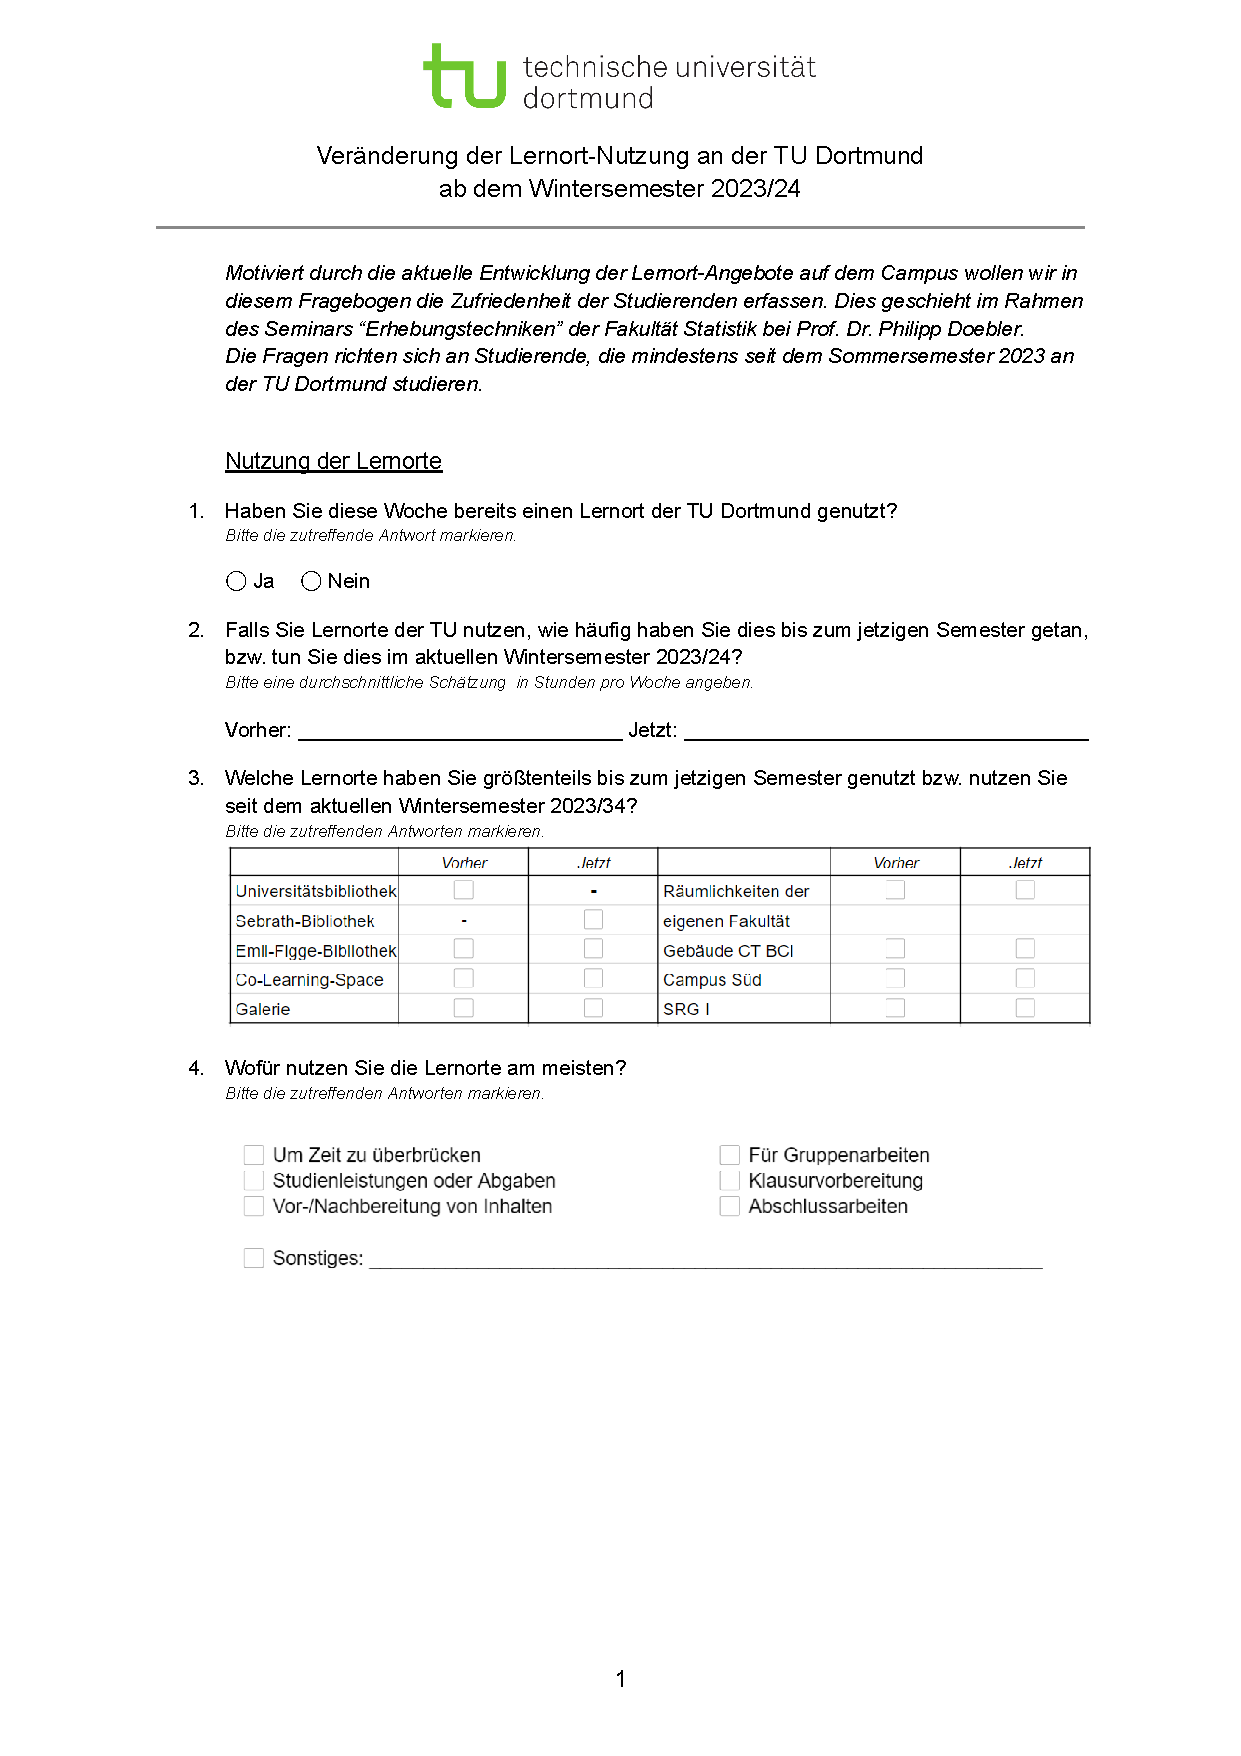
\includepdf[pages=1-4] {Fragebogen LJJY - 2023.pdf}
\newpage Appendix: Erklärung zu Anteilen an der Textproduktion

\end{document}



